\documentclass[a4paper, 12pt]{article}
\usepackage[a4paper,top=1.5cm, bottom=1.5cm, left=1cm, right=1cm]{geometry}
\usepackage{cmap}					
\usepackage{mathtext} 				
\usepackage[T2A]{fontenc}			
\usepackage[utf8]{inputenc}			
\usepackage[english,russian]{babel}
\usepackage{multirow}
\usepackage{graphicx}
\usepackage{wrapfig}
\usepackage{tabularx}
\usepackage{float}
\usepackage{longtable}
\usepackage{hyperref}
\hypersetup{colorlinks=true,urlcolor=blue}
\usepackage[rgb]{xcolor}
\usepackage{amsmath,amsfonts,amssymb,amsthm,mathtools} 
\usepackage{icomma} 
\usepackage{euscript}
\usepackage{mathrsfs}
\usepackage{enumerate}
\usepackage{caption}
\usepackage{enumerate}
\mathtoolsset{showonlyrefs=true}
\usepackage{graphicx}
\usepackage{caption}
\usepackage{subcaption}
\usepackage[europeanresistors, americaninductors]{circuitikz}
\DeclareMathOperator{\sgn}{\mathop{sgn}}
\newcommand*{\hm}[1]{#1\nobreak\discretionary{}
	{\hbox{$\mathsurround=0pt #1$}}{}}

\title{\textbf{Исследование взаимной диффузии газов (2.2.1)}}
\author{Манро Эйден}
\date{}

\begin{document}

\maketitle

\begin{center}
\section*{Введение}
\end{center}

\noindent \textbf{Цель работы:} 1) регистрация зависимости концентрации гелия в воздухе от времени с помощью датчиков теплопроводности при разных начальных давлениях смеси газов; 2) определение коэффициента диффузии по результатам измерений.

    \bigskip

    \noindent \textbf{Оборудование:} измерительная установка; форвакуумный насос; балон с газом  (гелий); манометр; источник питания; магазин сопротивлений; гальванометр; секундомер.

    \bigskip
    \begin{center}

\subsection*{Теоретические сведения}

{\sl Диффузия} - самопроизвольное взаимное проникновение веществ друг в друга, происходящее вследствие хаотичного теплового движения молекул. При перемешивании молекул разного сорта говорят о {\sl взаимной} (или {\sl концентрационной}) диффузии.
В системе, состоящей из двух компонентов, плотность потока вещества в результате взаимной диффузии описывается законом Фика:

\bigskip

\begin{center}
$\displaystyle j_a = -D_a_b\frac{\partial n_a}{\partial x}$, $\displaystyle j_b = -D_b_a\frac{\partial n_b}{\partial x}$,
\end{center}

\bigskip

где $D_a_b = D_b_a = D$ -- коэффициент взаимной диффузии компонентов, $j_{ab}$ = плотности потока частиц соответствующего сорта (количество частиц, пересекающих единичную площадку в единицу времени).\\
В работе исследуется диффузия примеси лёгкого газа (гелия) на фоне воздуха, поэтому концентрация воздуха в опыте значительно больше концентрации гелия, и её относительное изменение незначительно. В процессе работы будет описываться только диффузия примеси гелия на стационарном фоне воздуха.\\

Проведём теоретическую оценку величины коэффициента взаимной диффузии. В работа мала концентрация гелия, более того, масса атомов гелия много меньше массы молекул, составляющих воздух. При таких условиях перемешивание газов в эксперимента можно рассматривать как диффузию гелия на стационарном форне воздуха. Тогда коэффициент диффузии приблизительно равен
\begin{center}
$\displaystyle D = \frac{1}{3}\lambda \bar v$,
\end{center}
где $\lambda$ -- длина свободного пробега частиц гелия, $\displaystyle \bar v = \sqrt{\frac{8kT}{\pi m}}$ -- их средняя тепловая скорость. В общем случае необходимо считать $\displaystyle \lambda = \frac{1}{n_\Sigma \sigma}$, где $\displaystyle n_\Sigma = n_H_e + n_B = \frac{P_\Sigma}{kT}$ - полная концентрация частиц, $\sigma$ -- среднее сечение столкновения частиц гелия с воздухом. Также  $\displaystyle \bar v = \sqrt{\frac{8kT}{\pi \mu}}$ -- средняя относитель. Таким образом, теоретическая оценка предполагает, что коэффициент диффузии не зависит от пропорция элементов, а обратно пропорционален давлению $\displaystyle D \propto \frac{1}{P_\Sigma}$.
Рассмотрим процесс выравнивания концентрации в установке, она зависит от координат и времени во всей установке. Объём соединительной трубки мал по сравнению с с объёмами сосудов. Поэтому концентрации газов можно считать постоянной по всему объёму сосудов; считаем, что процесс выравнивания происходит только за счёт диффузии в трубке и является стационарным (так как считаем стационарным поток частиц). Величина этого стационарного потока $\displaystyle J = -DS\frac{\partial n}{\partial x}$, и он одинаковый во всём сечении трубки, тогда $n(x)$ - линейная функция координаты и $\displaystyle \frac{dn}{dx} = \frac{\triangle n}{l}$ (l -- длина трубки), получаем 
\begin{center}
$\displaystyle J = -DS \frac{n_1-n_2}{l}$.
\end{center}
Предположим, что установился линейный профиль концентрации и полученное соотношение справедливо в любой момент времени. Получаем {\sl квазистационарное} приближение зависимости концентраций $n_1$ и $n_2$ от времени.
\Через $\Delta n_1$ и $\Delta n_2$ обозначим изменения концентрации в объёмах $V_1$ и $V_1$ за время $\Delta t$. Тогда $V_1 \Delta n_1$ - изменение количества компонента в объёме $V_1$, а $V_2 \Delta n_2$ - изменение количества этого компонента в объёме $V_2$. По закону сохранения вещества следует, что $V_1 \Delta n_1 + V_2 \Delta n_2 = const$, поэтому $V_1 \Delta n_1 = - V_2 \Delta n_2$. Эти изменения происходят вследствие диффузии, поэтому 
\begin{center}
$\displaystyle V_1 \Delta n_1 = - V_2 \Delta n_2 = J \Delta t = -DS \frac{n_1-n_2}{l} \Delta t$
\end{center}
Делим равенство на $\Delta t$
\begin{center}
$\displaystyle V_1 \frac{dn_1}{dt} = -DS\frac{n_1-n_2}{l}$, $V_2 \frac{dn_2}{dt} = -DS\frac{n_1-n_2}{l}$
\end{center}
Делим первое уравнение на $V_1$, второе на $V_2$, вычтем равенства друг из друга:
\begin{center}
$\displaystyle \frac{dn_1}{dt}- \frac{dn_2}{dt} = - \frac{n_1-n_2}{l}DS(\frac{1}{V_1} +\frac{1}{V_2} )$.
\end{center}
Введём новую переменную $\Delta n = n_1-n_2$, проинтегрируем уравнение, получим
\begin{center}
$\Delta n = \Delta n_0 e^(^-^t^/^\tau^)$,
\end{center}
где $\Delta n_0$ - разность концентраций примеси в начльный момент времени, а
\begin{center}
$\displaystyle \tau = \frac{V_1 V_2}{V_1 + V_2} \frac {l}{SD}$.
\end{center}
Видим, что разность концентраций убывает по экспоненциальному закону и тем быстрее, чем меньше $\tau$ - величина, определяющаяся геометрическими параметрами установки и величиной коэффициента диффузии.
\item Для проверки применимости квазистационарного течения убедимся, что время $\tau$ много больше характерного времени диффузии одной частицы вдоль трубки длиной l: $\displaystyle t_{diff} \sim \frac{l^2}{D} \ll \tau$.

\item Для измерения концентраций применяются датчики теплопроводности $D_1$ и $D_2$ (см. рис. 1) и используется зависимость теплопроводности газовой смеси от её состава. Тонкая проволока радиуса $r$, протянутая вдоль оси цилиндра радиуса $R$, нагревается током. Тепло от проволоки к стенке цилиндра передаётся главным образом вспледствие теплороводности газа, находящегося внутри цилиндра. Количество тепла переданного стенке цилиндра в единицу времени, определяется по формуле 
\begin{center}
$\displaystyle Q = \kappa \frac{2\pi L}{ln (R/r)}(T_1-T_2)$,
\end{center}
где $\kappa$ - теплопроводность, $L$ - длина нити, $T_1, T_2$ - температуры проволочки и стенки. При $Q = const$ температура проволоки и её сопротивление определяются теплопроводностью газа и, следовательно, его составом. Для измерения разности концентраций газов используется  
мостовая схема, представленная на рис. 2 (см. пункт 4).

\item В процессе диффузии разность концентраций убывает по экспоненциальному закону. По тому же закону изменяются во времени показания гальванометра:
\begin{center}
$\displaystyle U = U_0 e^(^-^t^/^\tau^)$
\end{center}
Измеряя экспериментально зависимость $U(t)$, можно получить характерное время процесса $\tau$, откуда определить коэффициент диффузии D.

\begin{center}
\subsection*{Экспериментальная установка}
\end{center}

\item Общий вид конструкции установки приведён на рис. 1. Установка состоит из двух сосудов $V_1$ и $V_2$, соединённых краном $K_3$, форвакуумного насоса Ф.Н. с выключателем Т, манометра М и системы напуска гелия, состоящей из кранов $K_6, K'_6, K_7$. Кран $K_5$ позволяет соединять форвакуумны насос либо с установкой, либо с атмосферой. Сосуды $V_1$ и $V_2$ соединены трубкой длины $l$ и сечения $S$. Сосуды заполнены смесь двух газов при одинаковом давлении, но с различной концентрацией компонентов. Вследствие взаимной диффузии концентрации каждого из компонентов с течением времени выравниваются Между форвакуумным насосом и краном $K_5$ вставлен предохранительный баллон, защищающий кран и установку при неправильной её эксплуатации от попадания форвакуумного масла из насоса. Сосуды $V_1$ и $V_2$ можно соединять как с системой напуска гелия, так и с форвакуумным насосом. Для этот служат краны $K_1, K_2, K_4, K_5$. Манометр М регистрирует давление газа, до которого заполняют тот или иной сосуды. Кран $K_4$ изолирует форвакуумный насос от установки. Для подачи воздуха в установку служит кран $K_5$. Дополнительный кран $K'_6$ служит для вакуумной изоляции установки от системы подачи гелия. Краны $K_4, K_5, K'_6$ обладают повышенной вакуумплотностью и хорошо изолируют установку от протечек.

\begin{figure}[H]
    \centering
    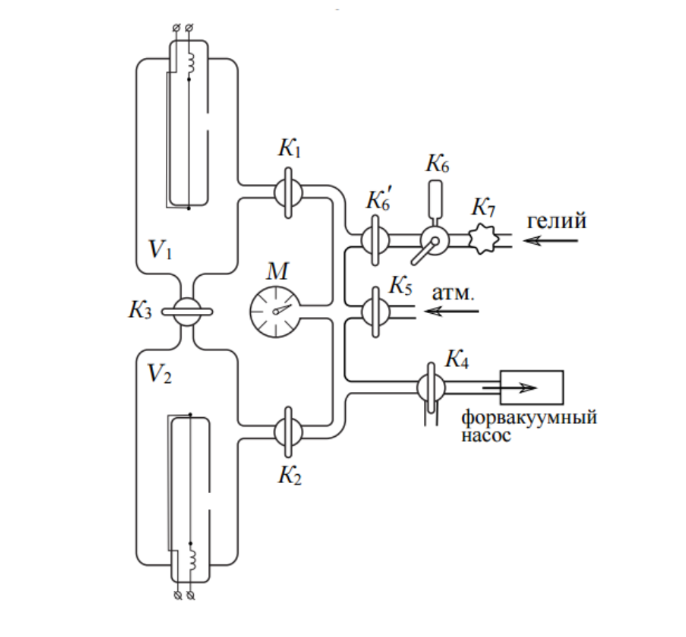
\includegraphics[width=9.5 cm]{facility.PNG}
    \caption{Установка для исследования взаимной диффузии газов}
    \label{fig:vac}
\end{figure}

\item Для измерения разности концентраций газов используется мостовая схема, представленная на рисунке 2. \\
Здесь $D_1, D_2$ - датчики теплопроводности, расположенные в сосудах $V_1$ и $V_2$. Сопротивления $R_1, R_2, R$ служат для установки прибора на нуль (балансировка моста). В одну из диагоналей моста включен гальванометр, к другой подключается небольшое постоянное напряжение. Сопротивления $R_1$ и $R_2$ спарены (их подвижные контакты находятся на общей оси) и изменяются одновременно при повороте ручки грубой регулировки. Точная балансировка выполняется потенциометром R. Балансировку необходимо проводить перед каждым экспериментом заново: при этом установка заполняется чистым газом (воздухом без гелия) при давлении, близком «рабочему» (при котором затем будут проводится измерения).

 Мост балансируется при заполнении сосудов (и датчиков) одной и той же смесью. При заполнении сосудов смесями различного состава возникает «разбаланc» моста. При незначительном различии в составах смесей показания гальванометра, подсоединённого к диагонали моста, будут пропорциональны разности концентраций примеси: $U \propto \Delta \kappa \propto \Delta n$
 
\begin{figure}[H]
    \centering
    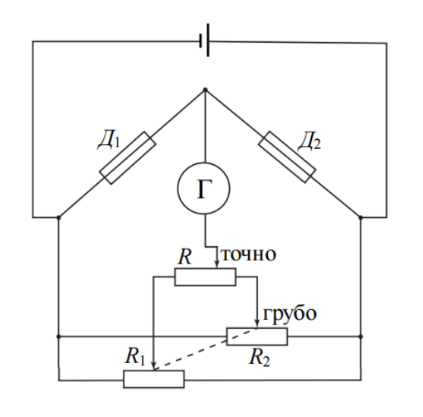
\includegraphics[width=7.5 cm]{scheme.PNG}
    \caption{Мостовая схема с датчиками теплопроводности для измерения разности концентраций газов}
    \label{fig:vac}
\end{figure} 

\item Гелий содержится в баллоне (не изображен на рис. 1) под давлением, превышающим атмосферное. Для предотвращения избыточного расхода гелия и
его неконтролируемого проникания в установку предусмотрен металлический кран (К7), отделяющий её от баллона с гелием. Его открывают только на
время непосредственного заполнения установки гелием, остальное время он должен быть закрыт. Для подачи малых порций гелия предусмотрен двухходовый кран с дозатором (рис. 4). При повороте рычажка Р в положение I гелий в небольшом количестве поступает в дозатор (если открыт К7), а при повороте Р в положение II порция из дозатора поступает в установку.

\begin{figure}[H]
    \centering
    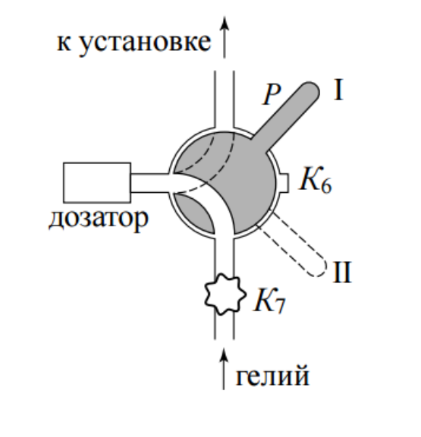
\includegraphics[width=6.5 cm]{crane.PNG}
    \caption{Кран $K_6$}
    \label{fig:vac}
\end{figure}

\section*{{Ход работы}

Все данные были сняты на компьютере и представляют собой более 2000 значений, в связи с чем их представление в работе не имеет смысла.

По полученным данным был построен график \ref{lnu(t)} зависимости логарифма напряжения от времени.

\begin{figure}[H]
    \centering
    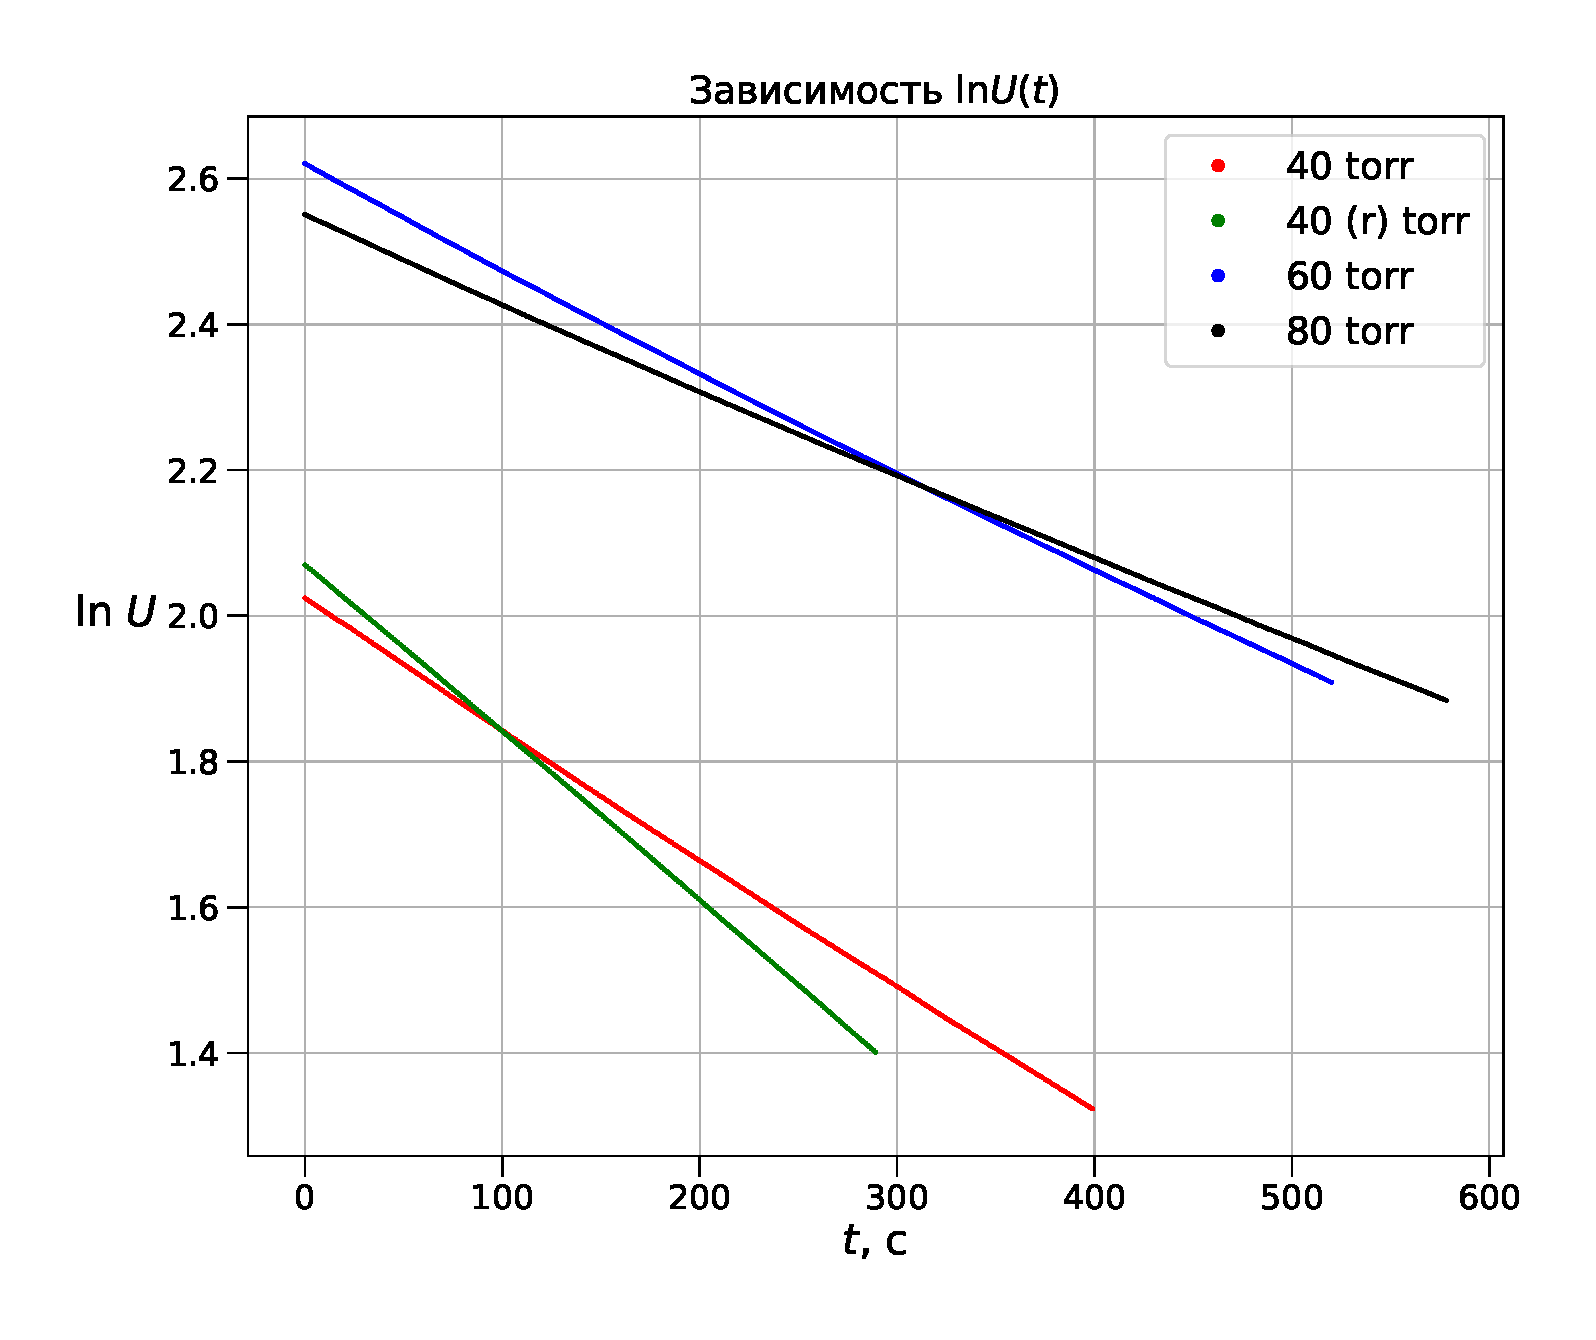
\includegraphics[scale=0.65]{lnu(t).pdf}
    \caption{Зависимость логарифма давления от времени}
    \label{lnu(t)}
\end{figure}

Коэффициент диффузии рассчитывается по формуле $\displaystyle D = -\frac{kVL}{2S}$, его ошибка будет составлять $\displaystyle \sigma_D = D\sqrt{\left(\frac{\sigma_V}{V}\right)^2+\left(\frac{\sigma_k}{k}\right)^2+\left(\frac{\sigma_L/S}{L/S}\right)^2}$.

Параметры установки: $V = 800 \pm 10\ \mbox{см}^3$, $L/S = (15,0 \pm 0,1)\ 1/$см.

\begin{center}
$\displaystyle     D_1 = 10,5 \pm 0,5\ \mbox{см}^2/\mbox{с},\ \sigma_{D_1} = 5\%$ \; ($P = 44$ торр)
\break

$\displaystyle     D_2 = 8,1 \pm 0,4\  \mbox{см}^2/\mbox{с},\ \sigma_{D_2} = 5\%$ \; ($P = 56$ торр)
\break

$\displaystyle     D_3 = 6,8 \pm 0,3\  \mbox{см}^2/\mbox{с},\  \sigma_{D_3} = 5\%$ \; ($P = 76$ торр)
\break

$\displaystyle     D_4 = 13,9 \pm 0,6\  \mbox{см}^2/\mbox{с},\  \sigma_{D_4} = 5\%$ \; ($P = 41$ торр (r))
\break

Построим графики зависимости коэффициента диффузии от величины, обратной давлению, отметим пределы погрешностей. Видно, что прослеживается обратная зависимость коэффициента диффузии от давления
\begin{figure}[H]
    \centering
    \begin{center}
    \caption{Зависимость коэффициента диффузии от величины, обратной давлению.}
    \end{center}
    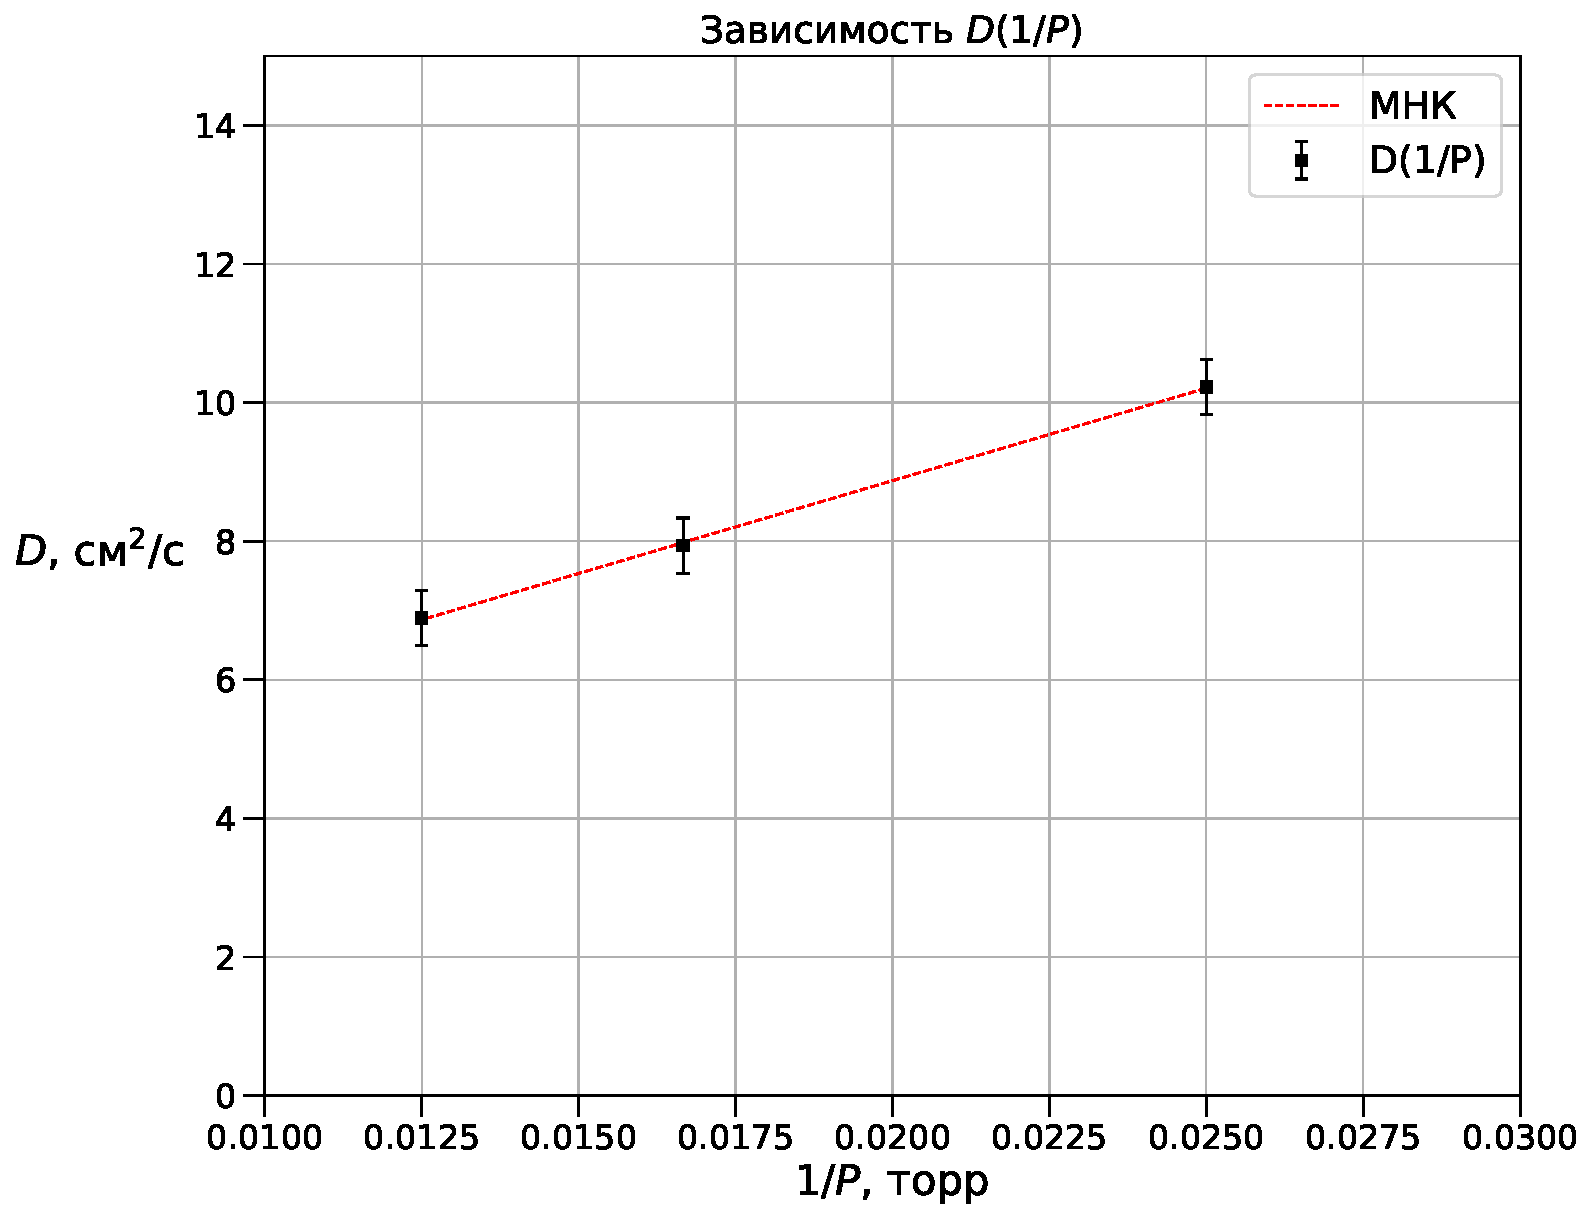
\includegraphics[scale=0.6]{d(p).pdf}
    \label{fig:vac}
\end{figure} 

Экстраполируя прямую значений, полученную нами, определим коэффициент диффузии гелия в воздухе при атмосферном давлении (760 Торр).\\
\begin{center}
$\displaystyle D_a = 0,76 \pm 0,07 \; \mbox{см}^2/$c - значения по расчётам \break

\end{center}

Сравним полученные значения с табличными. При температуре 273 К значение коэффициента диффузии примеси гелия в воздухе составляет $0.66 \ \mbox{см}^2/$c. Максимально приближенное к этому значение при расчётах с учётом максимальной возможной погрешности. Значения по компьютеру, по расчётам и по теории совпали по порядку величины, но не совпадают в пределах допустимой погрешности. 

Оценим длину свободного пробега молекулы по формуле:
\begin{center}
$\displaystyle \lambda = 3D \sqrt{\frac{\pi \mu }{8RT}} = 180,6 \pm 3,9$ нм
\break

\end{center}
При нормальных условиях табличное значение для длины свободного пробега молекулы гелия равно 180 нм. Экспериментальное и теоретическое значения совпали по порядку величины.

Наконец, оценим эффективное сечение столконевний атомов гелия с частицами воздуха при температуре 299 К и давлении $10^5$ Па:

\begin{center}
$\displaystyle \sigma = \frac{1}{\lambda n}$
\break

$\displaystyle \sigma = \frac{kT}{\lambda P} = (2,16 \pm 0,20) \cdot 10^{-19}$ м$^2$.
\end{center}


\section*{Вывод}

В ходе работы мо научились работать с форвакуумным насосом, а так же с вакуумным оборудованием. Убедились в том, что во время диффузии для концентраций газов выполняется соотношение  $\Delta n = \Delta n_0 e^{-\frac{t}{\tau}}$. Так же мы проверили, что коэффициент взаимной диффузии $D$ линейно зависит от обратного давления $1 / P$, при этом экстраполируя значения давления к атмосферному мы смогли получить приближенной значение $D_{атм}$. Так же используя величину $D_{атм}$ мы смогли получить оценки для длины свободного пробега атомов гелия $\lambda$ и  эффективного сечения столкновения в смеси воздух-гелий $\sigma_{\text{He-воздух}}$. 


\end{document}